\documentclass[12pt,draftcls,onecolumn]{IEEEtran}



\usepackage{amsmath,amssymb,amsthm}
\usepackage{mathrsfs}
\usepackage{verbatim}
\usepackage[english]{babel}
\usepackage{setspace}
\usepackage{graphicx}				
\usepackage{epstopdf}
\usepackage{amsmath}				
\usepackage{amssymb}
\usepackage{cite}
\usepackage{amsfonts}
\usepackage{enumerate}
\usepackage{amsthm}
\usepackage{array}
\usepackage{graphicx}
\setcounter{MaxMatrixCols}{48}
\usepackage{resizegather}
\usepackage{float}
\usepackage[section]{placeins}
\usepackage{fixltx2e}
\usepackage[justification=centering]{caption}
\usepackage{color}
\usepackage{lipsum} 
\usepackage{fancyhdr}
\usepackage{url}


\renewcommand\qedsymbol{}
\renewenvironment{proof}{{\bfseries Proof. }}{\textbf{Proof. }}
\newcommand{\RNum}[1]{\uppercase\expandafter{\romannumeral #1\relax}}
\usepackage{tikz}

\usetikzlibrary{arrows,positioning} 
\usepackage{verbatim}

 

\author{Zahra Gallehdari, Nader Meskin and Khashayar Khorasani
\thanks{This publication was made possible by NPRP grant No.  5-045-2-017
from the Qatar National Research Fund (a member of Qatar Foundation).
The statements made herein are solely the responsibility of the authors.}
\thanks{Zahra Gallehdari and Khashayar Khorasani are with the Department
of Electrical and Computer Engineering, Concordia University,
Quebec, Canada
         {\tt\small z\_galle@encs.concordia.ca} and  {\tt\small kash@ece.concordia.ca.}}
\thanks{Nader Meskin is with the Department of Electrical Engineering, Qatar
University, Doha, Qatar
        {\tt\small nader.meskin@qu.edu.qa.}}
}
\date{}

\renewcommand{\baselinestretch}{1.25}

\begin{document}


\title {\LARGE \bf 
An  Cooperative Fault Recovery Control   of Multi-Agent Systems}
\maketitle

\nocite{Basil:2010:MISC}

\newtheorem {lemmas}{\textbf{Lemma}} 
\newtheorem {theorems}{\textbf{Theorem}} 
\newtheorem {definitions}{\textbf{Definition}} 
\newtheorem {assumptions}{\textbf{Assumption}} 
\newtheorem {corollaries}{\textbf{Corollary}} 
\newtheorem{remarks}{\textbf{Remark}} 
\newtheorem{notations}{\textbf{Notation}} 
\newtheorem{Propositions}{\textbf{Proposition}} 
\newtheorem{facts}{\textbf{Fact}}
\newtheorem{algorithm}{\textbf{Algorithm}}


 \tikzset{
 	head/.style = {fill = orange!50!blue,
 		label = center:\textsf{\Large H}},
 	tail/.style = {fill = blue!70!yellow, text = black,
 		label = center:\textsf{\Large T}}
 }
\begin{abstract}
In this work, an  performance fault recovery control problem for a team of multi-agent systems that is subject to actuator faults is studied. Our main objective is to design a distributed control reconfiguration strategy such that \textbf{a)} in absence of disturbances the  state consensus errors either remain bounded or converge to zero asymptotically, \textbf{b)} in presence of actuator fault the output of the faulty system behaves exactly  the same as that of the healthy system, and \textbf{c)}  the specified   performance bound is guaranteed to be minimized in presence of bounded energy disturbances. 
The gains of the reconfigured  control laws are selected first by employing a geometric approach  where a set of controllers guarantees that the output of the faulty agent imitates that of the healthy agent and the consensus achievement objectives are satisfied. Next, the remaining degrees of freedom in the selection of the control law gains are used to minimize the bound on a specified  performance index. 
The effects of  uncertainties and imperfections in the FDI module decision in correctly estimating the fault severity as well as delays in invoking the reconfigured control laws are investigated and a bound on the maximum tolerable estimation uncertainties and time delays are obtained.
Our proposed distributed and cooperative control recovery approach is applied to a team of five autonomous underwater vehicles  to demonstrate its capabilities and effectiveness in accomplishing the overall team requirements subject to various actuator faults, delays in invoking the recovery control, fault estimation and isolation imperfections and unreliabilities under different  control recovery scenarios. 
\end{abstract}
\section{Introduction}
Utilization of unmanned vehicles (agents)  in operations where human involvement is dangerous, or impossible as in deploying mobile robots for planetary surface exploration, autonomous underwater vehicles for surveying  deep sea,  among others,  has  recently received extensive interest by the research community. In addition, deployment of multiple vehicles such as spacecraft, mobile robots,  or unmanned underwater vehicles instead of using  a single vehicle increases the  system performance and reliability, while it will ultimately reduce the cost of the overall mission. \par

 In safety critical missions, the agents should have the capability to  cope with unexpected external influences such as  environmental changes  or internal events such as actuator and sensor faults. If these unexpected events are not managed successfully, they can lead to the team  instability or cause sever overall team  performance degradations. For example, the crash of the NASA's DART spacecraft in 2006 was due to a fault in its position sensors  \cite{croomes2006}.\par 
 
The development of control reconfiguration for multi-agent systems is distinct from the control design problem of healthy multi-agent systems \cite{breger2008,Semsar2009,Ren2010a,Movric2014}. This is so in the sense that the former should be ideally solved on-line and use only local information given that faults  occur at unknown times, have unknown patterns,  and the existing fault detection and isolation (FDI) module in the team information may  be available only locally, while the latter problem can be solved  off-line and by potentially using the entire system  information. Moreover,  due to the  information sharing structure of multi-agent systems,  the fault tolerant control approaches that have extensively been studied in the literature for single agent systems  \cite{Yang2010,Wang2010,Liu2012,Xavier2012,Khosrowjerdi2004} \underline{will not be} directly applicable to multi-agent systems.\par

Recently, the control reconfiguration problem of multi-agent systems has been studied in  \cite{Tousi2012,Azizi11,ACC2014,ECC2014,Zhou2014,Zhao2014,Chen2014,Wang2015-2,Wang2015-3,Mehrabian2011,Mehrabian2011-2,Li2012,Xiao2013}. In \cite{Tousi2012,Azizi11}, formation flight problem in a network subject to loss of effectiveness (LOE) faults is considered and in  \cite{ACC2014,ECC2014,Zhou2014} the consensus achievement problem in faulty multi-agent systems is studied.  In  \cite{Tousi2012}, a discrete-event supervisory module is designed to recover the faults that cannot be recovered by the agents using only local recovery solutions. In \cite{Azizi11}, a  high-level performance monitoring  module is designed  that monitors all the agents and detects deviations of the error signals from their acceptable ranges. This module would then activate a high-level supervisor to compensate for the deviations in the performance specifications due to limitations of the low-level recovery strategy. In \cite{Zhao2014,Chen2014,Wang2015-2,Wang2015-3} adaptive control approaches are employed to compensate for actuator faults and in \cite{Mehrabian2011,Mehrabian2011-2} control reconfiguration problem in a team of Euler Lagrange systems subject to actuator faults and environmental disturbances is studied. Finally in \cite{Li2012,Xiao2013},  attitude synchronization problem for a team of satellites in presence of actuator faults is studied.  \par

In this work,   performance  control reconfiguration problem in multi-agent systems subject to occurrence of \underline{three} types of faults, namely, the loss of effectiveness (LOE), stuck and outage faults is studied. 
The proposed -based control reconfiguration  strategy  guarantees that the faulty agent outputs imitate those of the healthy system while  the state consensus errors are either ensured to be asymptotically stable or  remain bounded 
 in  absence of disturbances and  the disturbance attenuation bound is minimized when the disturbances exist. {Furthermore, this approach can compensate for the outage and stuck faults which cause rank deficiency and change the agent structure, whereas in the adaptive approaches it is assumed that the fault does not cause rank deficiency.  }
 
 Our proposed approach is similar to the works in \cite{Zhou2014, ECC2014}, but it has the following  distinctions, namely: (i) in \cite{Zhou2014} it is assumed that all the followers have access to the leader input signal while in this work {we do not} require this assumption,  (ii) in \cite{Zhou2014} environmental disturbances have not been considered whereas in this work {we do include} disturbances in our analysis and design, (iii) in this work agents could be subject to simultaneous LOE, outage and stuck faults, however in \cite{ECC2014} only a single LOE fault has been studied and in \cite{Zhou2014} only LOE and outage faults have been considered, (iv) in  both \cite{Zhou2014,ECC2014} the network topology is assumed to be indirected  whereas in this work we have considered a {directed network topology}, 
 and (v)  in this work we ensure that the outputs of the faulty agent are exactly  forced to follows those of the healthy agent and the state consensus errors remain bounded, whereas in \cite{Zhou2014,ECC2014} the consensus problem is considered. {The main motivation for enforcing outputs of the agents outputs to follow that of the leader is that in some applications like small light weight under vehicles, a small deviation in the speed can cause a big deviation in the agent position which may cause the network become disconnected or the agent becomes lost. In order to reach this objective, we formulated the problem as disturbance decoupling problem with stability and we use the Geometric approach \cite{Basile92} and controlled invariant subspaces to solve the problem along with linear algebra and matrix theory to address exact output following and state consensus error stability in the team as well as disturbance attenuation. To the best of our knowledge this problem has not been considered in the current literature in multi-agent systems.  }
 \par
 In view of the above discussion, the \underline{main contributions} of this work can be summarized as follows:
 \begin{enumerate}
 	\item [1)] A distributed control reconfiguration strategies for multi-agent systems subject to  LOE, outage and stuck faults are proposed and developed. Towards this end, associated with each agent a novel ``virtual auxiliary system'' is constructed for the first time in the literature. Each agent will receive information from {only} the states of its associated auxiliary agent and the nearest neighboring auxiliary agents. This is in contrast with conventional cooperative schemes where each agent will be receiving the actual state information from its nearest neighboring agents. The proposed strategy guarantee an  performance control reconfiguration with stability.
\item [2)] The proposed  reconfiguration control  laws  guarantee that 
	the output of the faulty agent behaves the same  as that of the healthy system, and  moreover a specified  performance index  is minimized  in presence of environmental disturbances.
 	\item [3)] The effects of  uncertainties and imperfections in the FDI module decision in correctly estimating the fault severity as well as delays in invoking the reconfigured control laws are investigated and a bound on the maximum tolerable estimation uncertainties and time delays are obtained.
 	\item [4)] The proposed distributed  reconfiguration control laws are capable of and designed specifically for accommodating single, concurrent and simultaneous actuator faults in multi-agent systems.
 \end{enumerate}
The remainder of this work is as follows. In Section \ref{section2}, the required background information are provided and the problem is formally defined. In Section \ref{proposed methodology}, the proposed reconfigured control law and the effects of uncertainties on the proposed solution are investigated. In Section \ref{simulation results}, the proposed control laws are applied to a network of Autonomous  Underwater Vehicles (AUV)s and extensive simulation results and various case studies are studied and presented. Finally, Section  \ref{conclusion} concludes the paper.
\section{ Background and Problem Definition}\label{section2}
\subsection{Graph Theory}\label{subsection 1.1}
 The communication network among  agents can be represented by a graph. A directed graph  consists of a nonempty finite set of vertices  and a finite set of arcs . The -{th} vertex represents the -{th} agent and the directed edge from  to  is denoted as the ordered pair , which implies that agent  receives information from agent . The neighbor set of the -th agent  in the network is denoted by . 
The adjacency matrix of the graph  is given by , where  if , otherwise . The Laplacian matrix for the graph  is defined as , where  and . 
\subsection{Leader-Follower Consensus Problem in a Network of Multi-Agent Systems}\label{subsection 1.2}
The main objective of the consensus problem in a leader-follower (LF) network architecture  is to ensure all the team members  follow the leader's specified  trajectory/states.
Consider a network with  follower agents that are governed by

and a leader  agent that has the dynamics given by

where {matrices , , ,  represent the agents dynamics matrices and  are known,}  , , , and ,  are the agents states, outputs, control signals, and  exogenous disturbance inputs. In this work,  bounded energy disturbances are considered, i.e. ,  ( belongs to  if   ).  

In the architecture considered in this paper, certain and \underline{a very few} of the followers, that are designated as \underline{pinned agents}, are communicating with the leader and receive data from it directly. The other \underline{followers are not in communication} with the leader and exchange information \underline{only} with their own nearest neighbor follower agents. {On the other word, each agent only communicate with its neighbors and at least one agent is a neighbour of the leader.}
The consensus error signal for the -th follower is now defined by
\begin{IEEEeqnarray}{rCl}
e_i(t)&=&g_{i0}(x_i(t)-x_0(t))+\sum_{j \in {\mathcal{N}_i}} (x_i(t)-x_j(t)),\label{agents consensus error}
\end{IEEEeqnarray}
where  if agent  is a pinned agent or is directly communicating with the leader and is zero otherwise. When there are no environmental disturbances, i.e. , ,  the team reaches a consensus if  converges to origin asymptotically as . However, when there exist environmental disturbances,   cannot converge to origin, although it should remain in a bounded region around the origin. We refer and designate both of these cases as achieving consensus through out this paper. 

{Based on the above representation for the network, the aim is that all follower agents follow the leader agent trajectory. Accordingly, we  partition the network Laplacian matrix defined in Subsection \ref{subsection 1.1}, 
as , , , where  is a  vector and represents the  leader's links to the followers and  is an  matrix and specifies the followers' connections. This will help us  to discuss the effects of the  leader agent and follower agents to reach the entire team objectives.}
\subsection{The Types and Description of the Actuator  Faults} 
Before formally defining the \underline{three} fault types that are considered in this work, we let  denote the matrix of  input channels of the healthy agent, where  denotes the -th column of the matrix ,   denote the matrix of the  faulty agent with a fault in only the -th input channel,  and  denote the matrix of the  faulty agent subject to several concurrent faulty channels. \\
\underline{\emph{Loss of Effectiveness (LOE) Fault}}: 
For the LOE fault, only a percentage of the generated control effort is available to the agent for actuation, therefore the dynamics of the -th faulty agent after the occurrence of a fault at  is modelled according to 

where  denotes the state of the faulty agent, , , for ,  represents the fault effectiveness  of the -th channel of the -th agent,  if the -th actuator is faulty, and  if it is healthy. \par
\noindent \underline{\emph{Outage Fault}}: If the -th actuator of the -th agent is completely  lost at the time , then we have  for , where . The dynamics of the -th agent with an outage fault in its -th actuator can be represented by 
 
where  .\par
\noindent \underline{\emph{Stuck Fault}}: If at the time  the -th actuator of the -th agent  freezes at a certain value and does not respond to subsequent commands, the fault is then designated as the stuck fault.  The dynamics of the -th faulty agent under this  fault type can be modelled as
 
where , and  for all  denotes the value of the stuck command. \par
We are now in a position to state the following assumptions. 
\begin{assumptions}\label{network structure}
(a) The network graph is directed and  has a spanning tree, and 
(b) The leader control input is bounded and the upper bound is known.
 \end{assumptions}
 \begin{assumptions}\label{assumption 2}
(a) The agents are stabilizable and remain stabilizable even after the fault occurrence.\\
(b) Each agent is equipped with a local FDI module which detects with possible delays and correctly isolates the fault in the agent and also estimates the severity of the fault with possible errors in the case of the LOE or stuck faults. 
\end{assumptions}
Regarding the above assumptions the following clarifications are in order. First, the Assumptions \ref{network structure}-(a) and  \ref{assumption 2}-(a)  are  quite common   for consensus achievement and fault recovery control design problems, respectively.   
Second, it is quite necessary that in most
practical applications one considers a leader whose states
are ensured to be bounded. Moreover, in practical scenarios
the actuators are quite well understood and described
and their maximum deliverable control effort and bound they can tolerate are readily available and known. Therefore Assumptions \ref{network structure}-(b) is also not  restrictive. Furthermore, in Subsection \ref{subsection 3} we analyze the system behavior for situations where either Assumption \ref{assumption 2}-(c) does not hold or 
  the estimated fault severities by the FDI module are not accurate. We obtain the maximum uncertainty bound that our proposed approaches can tolerate.  However, as stated in Assumption \ref{assumption 2}-(b),  we require the correct actuator location  as well as the type of the fault for guaranteeing that our proposed reconfigured control laws will yield the desired design specifications and requirements. The Scenario  in Section \ref{simulation results} does demonstrate the consequences of violating this assumption.
 
 As far as Assumption 2-(c) is concerned, it should be
noted that this assumption is indeed quite realistic for
the following observations and justications. The transient
time that any cooperative or consensus-based controller
takes to settle down and the overall team objectives
are satisfied is among one of the design consideration
and specification for the controller selection. In most
practical consensus achievement scenarios dealing with a healthy team, the transient time associated with the
agent response is ensured to be settled down in a very
small fraction of the entire mission time, and in most
cases the healthy transient time takes a few seconds to
minutes to die out. Therefore, it is quite realistic and
indeed practical that during this very short and initial
operation of the system, the agents are assumed to be
fault free. In other words, we will not initiate the mission
with agents that are faulty from the outset. It is highly
unlikely that during the very first few moments after the
initiation of the mission a fault occurs in the agents. For
all the above explanations and observations we believe
that Assumption 2-(c) is meaningful and quite realistic.
\subsection{Notations and Preliminaries}
For a vector  we define  ,  (Euclidean norm ) and  norm as , , . The signal  is also represented as . The function  is defined as

 For the vector  the notation  denotes a diagonal matrix that has diagonal entries 's. The notations ,  and  denote  an identity matrix of dimension , a unity  vector with all its entries as one, and a zero matrix of dimension , respectively. For a matrix , the notation  () or  () implies that  is a positive definite (positive semi-definite) or a negative definite (negative semi-definite) matrix. For a matrix , its -norm is defined by 
 
  The term  () denotes the generalized left (right) inverse of the matrix . The terms ,  and  denote the -th  eigenvalue, the smallest, and the largest eigenvalues of the matrix , respectively. For the matrix , , , ,  denote the -th  singular value, the minimum singular value, and the largest singular value of . 
The notations  and   denote the image and the kernel of . 
\begin{theorems}\label{theorem 0.3}\cite{Yedavalli14}
Consider the system 

where  is Hurwitz stable and  is the state vector. The system (\ref{eq 0.10}) is stable if 

for all  and , where  is the solution to 

\end{theorems}
\begin{facts}\label{Fact1}
For any two matrices  and  and a positive scaler  we have 

\end{facts}
\subsection{Problem Definition}\label{subsection 2-E}
 In this work, our main goal and objective is to design a state feedback reconfigurable  or recovery control strategy in a directed network of multi-agent systems that seek consensus in presence of three types of actuator faults and environmental disturbances. 
 Suppose the -th agent becomes faulty and its first  actuators are subject to the outage fault,  to  actuators are subject to the stuck fault, while the remaining  actuators are either subject to the LOE fault or are healthy. Using equations (\ref{faulty system})-(\ref{LIP}) the model of -th faulty agent that is subject to three types of actuator faults can be expressed as
 
where  
, , , 
,  , ,  denotes the -th actuator effectiveness and fault severity factor, , , . \par
Considering the structure of the control law  and the matrix , it follows that only  the actuators  to  are available to be reconfigured. Therefore, to proceed with our proposed control recovery strategy the model (\ref{faulty system pre.}) is rewritten as follows 
 \par
The main objective of the control reconfiguration or control recovery is to design and select     such that the state consensus errors either remain bounded and ,  for , when , , and the environmental disturbances are  attenuated for , where , , and  is defined as in equation (\ref{LL or F}).\par 
 To develop our proposed reconfiguration control laws, a \textbf{\underline{virtual auxiliary system}} associated with each agent is now introduced as follows
 
where ,  and  denote the state of the auxiliary system corresponding to the -th agent,  its control and output signals, respectively.  
Furthermore, the disagreement error for each auxiliary system is also defined as
 
 The auxiliary system that is defined in (\ref{aux LF dynamics}) is ``virtual" and is not subject to actuator faults or disturbances, and hence it can be used as the {reference model} for designing the reconfigured  control laws of the actual  system (\ref{LL or F}) once it is subjected to actuator faults.\par 
 The   performance index corresponding to the -th healthy agent (\ref{LL or F}) and the -th faulty agent (\ref{faulty system 2}) is now defined according to 
 
 where 
, 
 and  and  represent the disturbance attenuation bounds. Based on the above definitions, the team performance index is now defined by . Under the control laws , , the  performance index bound for the healthy team is attenuated if , .  Furthermore, the  performance index for the -th faulty agent is attenuated if , , . {It should be noted that
 the performance indices (\ref{agent cost index}) and (\ref{auxiliary cost index}) are not and cannot be calculated directly as the disturbance is unknown and the aim of the proposed approach is to minimize the performance indices without directly calculating them.}
 
We are now in a position to formally state  the problem that we consider in this work.
 \begin{definitions}\label{def. 1}
 (a) The   state consensus  performance control problem for the  healthy  team is solved if in  absence of  disturbances, the agents   follow the leader states and consensus errors converge to zero asymptotically, and in  presence of disturbances, the prescribed   performance bound for the healthy team is attenuated, i.e. .\\ 
 (b) Under Assumptions \ref{network structure} and \ref{assumption 2}, the  performance  control reconfiguration problem with stability is solved if in absence of  disturbances the state consensus errors remain bounded  
 while the output of the faulty agent behaves the same as those of the healthy system outputs, and in presence of disturbances the disturbance attenuation bound is minimized and .
 \end{definitions}
\section{ Performance Cooperative and Distributed  Control Reconfiguration Strategy}\label{proposed methodology}
In this section, our proposed  reconfigurable control law is introduced and developed.  Since each agent only shares its information with its nearest neighbors,  the reconfiguration control strategy also employs the same information as well as the agent's FDI module information. \par
Consider the dynamics of the -th faulty agent is given by (\ref{faulty system 2}). As defined above  ,  with  denoting the -th faulty agent  state and   defined in (\ref{aux LF dynamics}),  we let  to  denote the deviation of the output of the faulty agent from its associated auxiliary agent output. Then, the dynamics associated with  can be obtained as

Moreover, the faulty agent consensus error is defined as 

\begin{lemmas}\label{Lemma 1}
The faulty agent consensus error (\ref{cons. er}) is stable 
if  and  are asymptotically stable and  is stabilized.
\end{lemmas}
\proof
From the auxiliary error dynamics  (\ref{eq. 1.11}), one can express the state consensus error dynamics for the -th faulty agent that is denoted by  according to

Therefore if the control law  can be reconfigured such that  is stabilized then it follows that  will be stable. This completes the proof of the lemma.   \qed
\par
The above lemma shows that stability of the faulty agent's consensus error can be guaranteed by  reconfiguring the control law  such that   is stable. This implies that  one can transform the control reconfiguration problem to that of the stabilization problem. Consequently, in the next two subsections we consider the problem of stabilizing . However, as  seen from (\ref{eq. 1.11}), the dynamics of  depends on the control of the healthy agents. Hence, before presenting our proposed control reconfiguration strategy, the control law for   the healthy team (where it is assumed without loss of any generality that all the agents are healthy) is presented below.
 \par
In this work, the following general  control law structure is utilized,

which is the generalization of the one  developed in \cite{Li13} and is given by 

where , and   and  are given by (\ref{auxiliary consensus}) and (\ref{agents consensus error}), respectively.

\begin{remarks}
The main challenge in developing the reconfigurable control law in multi-agent system as compared to that in single agent is that  in single agent control recovery the agent is redesigned its control law to maintain its stability. However, in multi-agent system the agent should redesign its control law such that the entire team remains stable and loosing one agent can cause a disconnected network and failing the entire mission. The main difficulty  in the design which is not the case in single agent is that   each agent only share information with its nearest neighbours and communication channels are limited, so that the design should be performed using only local information.  
\end{remarks}

The followings comments summarize the main characteristics of  the control law (\ref{proposed healthy control law}) : 

\textbf{(1)} In the control law (\ref{proposed healthy control law}) an agent employs and communicates \underline{only} the auxiliary states  that are   unaffected by  both disturbances and  faults. 
In contrast  in standard consensus control schemes such as  (\ref{Li control law})  the actual states  are employed and communicated from the nearest neighbor agents.  
 Hence, the utilization of  (\ref{proposed healthy control law})   avoids the propagation of the adverse effects of the disturbances and faults  through out the team of multi-agent systems. This along with the degrees of freedom in designing the control recovery laws  allow us to manage the -th faulty agent by {only} reconfiguring the control law of the faulty agent, and moreover it also provides us with the capability to recover simultaneous faults in multiple agents. 
 
  \textbf{(2)} The gain  is designed such that the states of the -th agent follow the states of its associated auxiliary agent,  while the gain  is designed such that the states of the auxiliary agents reach a consensus and follow the leader state. 
\footnote{The states  are virtual; however, since  depends on the leader state,  also depends on the leader state  (which is  available to only a very few follower agents in the network). Therefore,  should be communicated between the neighboring agents.}  
\par
\textbf{(3)} Each agent receives only the auxiliary agents states in its nearest neighbor set as opposed to  their actual states 
 that is conventionally required in standard multi-agent consensus approaches. 
 
 \textbf{(4)} The control law (\ref{proposed healthy control law}) is shown subsequently to solve the consensus problem in a \underline{directed} network topology that is {subject to environmental disturbances}, whereas the control law (\ref{Li control law}) solves the consensus problem in {disturbance free} environment and where the network topology is assumed to be \underline{undirected}. The procedure for selecting and designing the gains of the control law (\ref{proposed healthy control law}) is provided in Theorem \ref{theorem 1}.  Moreover, 
the structure of the proposed control law of this agent are provided in Figures \ref{network schematic} and \ref{ith agent control schematic}. \begin{theorems}\label{theorem 1}
	The control law 
	
	 solves the  performance state consensus problem in a team of  follower agents whose dynamics are given by (\ref{LL or F}) and the leader dynamics that is given by (\ref{L1}), if  and  are selected as follows:
	
	 where  is  defined as in (\ref{auxiliary consensus}), 
	, , ,  is  defined as in (\ref{sgn}), ,   , and finally the positive definite matrix  is the solution to
	
	and  and  are solutions to
	
	where  denotes the number of pinned agents,  is the desired disturbance attenuation bound,  ,   
	and 's are the solutions to the inequalities
	
	where  denotes the upper bound of the leader control signal, i.e.,  for all .
\end{theorems}
\proof
The team reaches a consensus if . This goal is also achieved if agents' controls are designed such that  () and  () for . 
This implies that the consensus achievement problem can be re-stated as  the problem of asymptotically stabilizing  
 and  simultaneously. \par
In the following, first we discuss the stability criterion and disturbances attenuation for   and  in Parts A and B, respectively and  then in Part C, we derive the conditions that  satisfy the requirements for both Parts A and B that in fact solve the  performance state consensus.\par
\underline{\textbf{Part A}}: From  (\ref{aux LF dynamics}) and (\ref{auxiliary consensus}), the dynamics of  can be obtained as 

where  , , , , . Let us select   as , then the system (\ref{eq. 2.1}) becomes

where  and . Since the  function is discontinuous, in order to conduct  the stability analysis of the system  (\ref{augmented error auxiliary}), it is replaced with its differential inclusion (for more details refer to \cite{Shevitz94,Bacciotti99}) representation as follows 

where the operator  is defined as in \cite{Shevitz94,Bacciotti99} to investigate its Filipov solutions. Now,  we require to define the Lyapunov function candidate  to study the stability properties of the error dynamics system. 
For this purpose, let us select , as a Lyapunov function candidate for the system (\ref{augmented error auxiliary 1}), where . Also, let , so that 
the set-valued derivative of  along the trajectories of the system (\ref{augmented error auxiliary 1}) is given by 
\par
Let , ,  and . Since  is a scaler, , and one has 

Then by using the Holder's inequality 

where  is the -th element of  and we use the fact that .  
On the other hand,   can be written as

where 
\par
Let , then three cases can be considered depending on the value of  as follows:\\
i) , then .\\
ii) , then . Since  and , it follows that

and if ,  are designed such that , then 

iii) , then  and . Therefore,

Again if ,  are designed such that, , then
\par
Let . From the  inequalities  (\ref{eq 15.1})-(\ref{eq 2.14})  it follows that

Suppose that s and  are obtained such that
 
Now by using the Fact \ref{Fact1} for the last term in the right-hand side of  (\ref{eq. 6.5}) with ,  and , and also the inequalities (\ref{eq 2.17}) and (\ref{eq. 1.12}), the expression (\ref{eq. 6.5}) can be replaced with the following inequality
\par
Since now the right hand side of the above inequality is continuous, the operator  can be removed. Let   and add  to both sides of the above inequality then it follows that 

where

From \cite{Shevitz94}, we require   to be negative definite, which will be achieved if  is obtained such that

and  are selected such that

Therefore, if ,  and  are selected as the solutions to (\ref{eq 2.18}) and (\ref{eq. 1.1}),  the function  will be negative definite  and for , it follows that  , or equivalently the consensus errors are asymptotically stable. \par
Now, if the initial conditions are set to zero and the disturbance is the only input to the agents, then by integrating the left-hand side of (\ref{eq 2.19}) one gets 

Given that , 
		  and ,   it follows that  

where  and .  Hence, from the inequalities (\ref{eq. 1.2}) and (\ref{eq. 1.3}) it follows that  

and by selecting  one gets  
\par
\underline{\textbf{Part B}}: Under our proposed  control law the dynamics of the -th auxiliary agent tracking error, , can be expressed as 

Consider  as a Lyapunov function candidate for the system (\ref{error tracking 1}) and  select . It then follows that 

and by following along the same steps as in Part A, the above equality can be written as 

Now if  is obtained such that 

then . This implies that for , we have , and for , one gets

\underline{\textbf{Part C}}: In order to obtain the positive definite matrix  that satisfies the inequalities (\ref{eq. 1.1}) and (\ref{eq 1.5}) and also guarantees the disturbance bound attenuation, let us set   and  as  and , respectively. Given that , it can be observed that if  satisfies 

then inequalities (\ref{eq. 1.1}) and (\ref{eq 1.5}) will both hold, where  is the solution to (\ref{eq. 1.12}). 
On the other hand

Now from equations (\ref{eq. 1.6}) one has

and by using  (\ref{eq. 1.13})

then it follows that 

Therefore, the team  performance upper bound can be expressed as

The above inequality implies that , or equivalently the healthy team  performance criterion holds. This along with the  properties of the stability of  and , as stated in Parts A and B, imply that our proposed control law solves the  performance state consensus problem for the healthy team. \qed
\begin{figure}
	\centering
{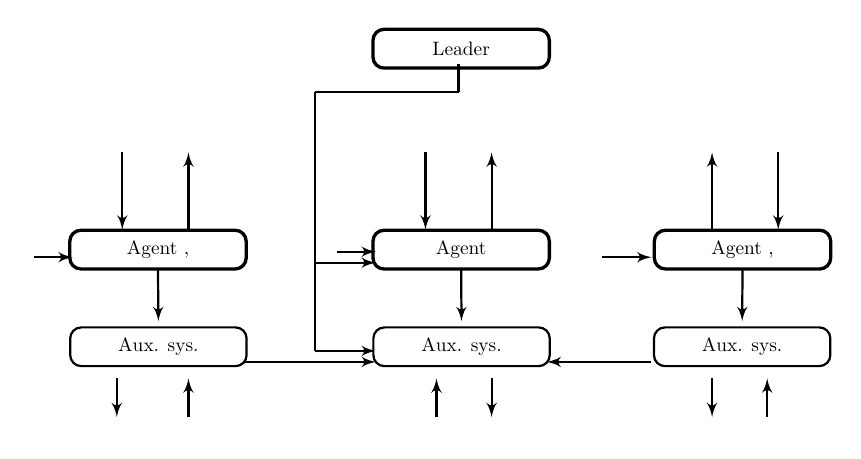
\begin{tikzpicture}[thick,scale=0.7, every node/.style={transform shape}]
		[node distance=1cm, auto]  
		\tikzset{
mynode/.style={rectangle,rounded corners,draw=black, top color=white, bottom color=white,very thick, minimum height=2em,  minimum width=3.2cm, text centered},
			mynode1/.style={rectangle,rounded corners,draw=black, top color=white, bottom color=white, minimum height=2em,  minimum width=3.2cm, text centered},		
			myarrow/.style={->, >=latex', shorten >=2pt, thick},	
			myarrow2/.style={<-, >=latex', shorten >=2pt, thick},
			myarrow3/.style={->, >=latex', shorten >=2pt, dashed},		
			myarrow4/.style={<-, >=latex', shorten >=2pt, dashed},
			myarrow5/.style={<-, >=latex', shorten >=2pt, dashed},			
			mylabel/.style={text width=7em, text centered} 
		}  
		\node at (0,-0.2) (leader) {};  
		\node[ below=2.5cm of leader] (cen1) {}; 
		\node[mynode, left=6.3cm of cen1] (agentk) {Agent ,  }; 
		\node[mynode, left=0.8cm of cen1] (agent2) {Agent };
		\node[mynode, right=0.8cm of cen1]  (agent3) {Agent , };
		\node[ mynode,  above=2.9cm of agent2] (Leader) {Leader}; 
            \draw  (-5.2,-0.1)  --  (-2.6,-0.1);
            \draw  (-2.6,-0.1)  --  (-2.6,0.4);            
            \draw  (-5.2,-0.1)  --  (-5.2,-4.8);
            \draw[myarrow]  (-5.2,-3.2)  --  (-4,-3.2);
            \draw[myarrow]  (-5.2,-4.8)  --  (-4,-4.8);
		\draw[myarrow]  (-8.7,-1.2)  --  (-8.7,-2.7);
		\node[above] at (-8.7,-1.2)	{ };	
		\draw[myarrow2]  (-7.5,-1.2)  --  (-7.5,-2.7);
		\node[above] at (-7.5,-1.2)	{ };	
		\draw[myarrow]  (-10.3,-3.1)  --  (-9.5,-3.1);
		\node[above] at (-10.3,-3.2)	{ };	
		
		\draw[myarrow]  (-3.2,-1.2)  --  (-3.2,-2.7);
		\node[above] at (-3,-1.2)	{ };	
		\draw[myarrow2]  (-2,-1.2)  --  (-2,-2.7);
		\node[above] at (-2,-1.2)	{ };	
		\draw[myarrow]  (-4.8,-3.0)  --  (-4.0,-3.0);
		\node[above] at (-4.6,-2.95)	{ };	
		
		
		\draw[myarrow]  (3.2,-1.2)  --  (3.2,-2.7);
		\node[above] at (3,-1.2)	{ };	
		\draw[myarrow2]  (2,-1.2)  --  (2,-2.7);
		\node[above] at (2,-1.2)	{ };	
		\draw[myarrow]  (0,-3.1)  --  (1,-3.1);
		\node[above] at (0.5,-3.2)	{ };	
		
		
		\node[ below=1.5cm of leader] (cen2) {};				
		\node[ below=1.5cm of cen1] (cen3) {}; 
		\node[mynode1, left=6.3cm of cen3] (auxk) {Aux. sys. }; 
		\node[mynode1, left=0.8cm of cen3] (aux2) {Aux. sys. };
		\node[mynode1, right=0.8cm of cen3]  (aux3) {Aux. sys. };
		\draw[myarrow] (agentk.south)  --  (auxk.north);
		\draw[myarrow] (agent2.south)  --  (aux2.north);
		\draw[myarrow] (agent3.south)  --  (aux3.north);

		\draw [myarrow2] (-1,-5.0) -- (+1,-5.0);
		\node[above] at (0,-4.9)	{};
		\draw [myarrow] (-6.5,-5.0) -- (-4,-5.0);
		\node[above] at (-4.6,-4.95)	{ };		
		
		\draw[myarrow2] (-8.8,-6.0)  --  (-8.8,-5.2);
		\node[below] at (-8.8,-6.0)	{ };
		\draw[myarrow]  (-7.5,-6.0)  --  (-7.5,-5.2);
		\node[below] at (-7.5,-6.0)	{ };			
		
		\draw[myarrow2] (-2,-6.0)  --  (-2,-5.2);
		\node[below] at (-2,-6.0)	{ };
		\draw[myarrow]  (-3,-6.0)  --  (-3,-5.2);
		\node[below] at (-3,-6.0)	{ };
		
		\draw[myarrow2] (2,-6.0)  --  (2,-5.2);
		\node[below] at (2,-6.0)	{ };
		\draw[myarrow]  (3,-6.0)  --  (3,-5.2);
		\node[below] at (3,-6.0)	{ };
		
		\end{tikzpicture}} 
	\caption{The schematic of the -th pinned agent and its nearest neighbor agents  and , which are not pinned.
	} 
	\label{network schematic}
\end{figure}

\begin{figure}
	\centering
{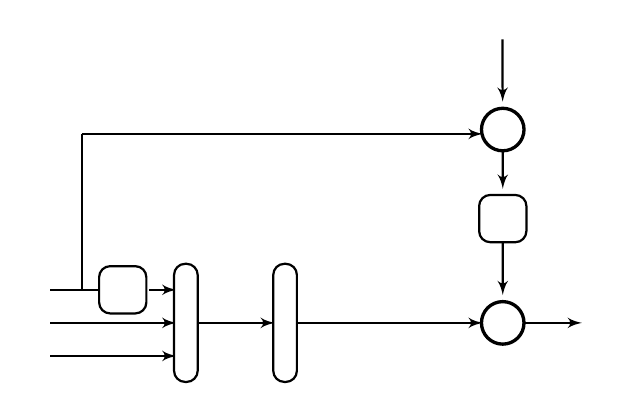
\begin{tikzpicture}[thick,scale=0.6, every node/.style={transform shape}]
		[node distance=1cm, auto]  
		\tikzset{
			mynode/.style={rectangle,rounded corners,draw=black, top color=white, bottom color=white,very thick, minimum height=2em,  minimum width=3.2cm, text centered},
			mynode1/.style={rectangle,rounded corners,draw=black, top color=white, bottom color=white, minimum height=2.5cm,  minimum width=0.5cm, text centered},	
			mynode2/.style={circle,draw=black, very thick, minimum size=0.9cm, text centered},	
			mynode3/.style={rectangle,rounded corners,draw=black, top color=white, bottom color=white, minimum height=1cm,  minimum width=1cm, text centered},						
			myarrow/.style={->, >=latex', shorten >=2pt, thick},	
			myarrow2/.style={<-, >=latex', shorten >=2pt, thick},
			myarrow3/.style={->, >=latex', shorten >=2pt, dashed},		
			myarrow4/.style={<-, >=latex', shorten >=2pt, dashed},
			mylabel/.style={text width=7em, text centered} 
		}  
		
		\draw[myarrow2] (-0.2,0.7)  --  (-0.9,0.7);	
		\draw[myarrow2] (-1.5,0.7)  --  (-3,0.7);	
		\node[left] at (-3.1,0.7)	(label xi) {   };
		\node[mynode3, right=1.25cm of label xi] (gain2){};				
		\draw[myarrow2] (-0.2,0)  --  (-3,0);
		\node[left] at (-3.1,0)	{};			
		\draw[myarrow2] (-0.2,-0.7)  --  (-3,-0.7);
		\node[left] at (-3.1,-0.7)	{ };		
\node[mynode1] (sum1) {};  
		\node[ left=-0.3cm of sum1] (cen1) {}; 
		\node[mylabel, above= 0.3cm of cen1] (label1) { };
		\node[mylabel, above= -0.5cm of cen1] (label2) { };		 
		\node[mylabel, above= -1.1cm of cen1] (label2) { };	
		
		\draw[myarrow] (sum1)  --  (2.0,0);
		\node[above] at (1.0,0)	{ };
		
		\node[mynode1, right=1.8cm of cen1] (aux2) (aux cont){};	
		\draw[myarrow] (aux cont)  --  (6.4,0);
		\node[above] at (5.7,0)	{ };
		\node[above] at (7.1,0.5)	{ };	
		\node[above] at (6.0,-0.65)	{ };	
		
		\node[mynode2, right=6.2cm of cen1] (sum2){};	
		\draw[myarrow] (sum2)  --  (8.5,0);
		\node[right] at (8.5,0)	{ };
		
		\draw[-] (-2.2,0.7)  --  (-2.2,4.0);
		
		\draw[myarrow] (-2.2,4)  --  (6.4,4);		
		\node[mynode2, above=3.15cm of sum2] (sum3){};
		\node[mynode3, below=0.9cm of sum3] (con2){};	
		\draw[myarrow] (sum3)  --  (con2);
		\draw[myarrow] (con2)  --  (sum2);			
		\draw[myarrow] (6.7,6)  --  (sum3);
		\node[above] at (6.7,6)	{ };	
		\node[right] at (6.7,5.1)	{ };	
		\node[right] at (5.5,4.3)	{ };		
		\node[right] at (6.8,3.4)	{ };							
		\end{tikzpicture}} 
	\caption{The -th agent cooperative control structure and its associated auxiliary system control laws, where   and  is defined in (\ref{auxiliary consensus}).} 
	\label{ith agent control schematic}
\end{figure}
\subsection{ Performance Control Reconfiguration}\label{subsection 1}
Consider the representation of an agent subject to presence of faults be  specified as in Subsection \ref{subsection 2-E}, and given by the equation (\ref{faulty system 2}) or equivalently by the transformed model (\ref{eq. 1.11}). Our proposed reconfigured control law for the -th faulty agent is now given by

{where  ,  are control gains and  is the control command to be designed later}. Therefore the dynamics of the closed-loop faulty agent (\ref{eq. 1.11})  becomes 
\par
 As per Definition \ref{def. 1}, the  control reconfiguration objectives can now be stated as that of selecting the gains  and  and the control command  such that (a)  is stable, (b)  (that is, ) for , , and  (c)   for .  In order to pursue the reconfiguration strategy we required the following assumption, we later discuss how deviation of this assumption affect the results.
{ \begin{assumptions}\label{stuck condition1}
 Under the fault scenario, there still enough actuator redundancy to compensate for the fault, i.e.

\end{assumptions}
 then there exists a control signal   such that }
  
 Subject to the above condition, equation (\ref{faulty agent tracking}) now becomes
\par
 Let us  temporarily assume that  , then
 
{ From (\ref{eq. 2.3}), to ensure that the outputs of the faulty agent do not deviate after fault, both terms should be zero or negligible. The first term will be negligible if the agents reach a consensus before fault occurrence i.e.  or if   is designed such that   damps very fast.  This can be  achieved easily if  is small enough. }
On the other hand,   according to Theorem \ref{theorem 1}, . Given that the control gains are designed such that  is asymptotically stable and  is bounded,   also remains bounded.  Considering that  does not depend on the dynamics of , it can be treated as a disturbance to the system (\ref{faulty agent tracking 2}).  
Consequently, the problems of \emph{(i)} enforcing  (for , ,  and any ), and \emph{(ii)} stabilizing  ,  is similar to that of the disturbance decoupling problem with stability (DDPS), as studied in \cite{Lunze2006}. \par
 The geometric approach that is based on the  theory of subspaces \cite{Basile92} is the most popular method for solving the DDPS problem. Towards this end, we first  introduce the required subspaces as follows:
 , ,  and  denote the maximal  controlled invariant  subspace that is contained in , and the maximal \underline{ internally stable}  controlled invariant  subspace that is contained in , respectively. \par
 Following the procedure in \cite{Basile92}, if  and  are selected such that 
 
 then  the second term in (\ref{eq. 2.3}) will also vanish. On the other hand, if  and  are selected such that 
  
 then the second term in (\ref{eq. 2.3})  will also vanish and  will be stable due to the stability of the subspace .
Unfortunately, there is no systematic approach to explicitly obtain , implying that  cannot be computed and employed directly for obtaining  that satisfies the condition (\ref{DDPS}). Therefore, we are required to transform the  condition (\ref{DDPS}) into a verifiable one. Once such a controller is obtained, one can then ensure that  and  will remain stable. \par
Given that  is  controlled invariant, \underline{there exists a matrix , a friend of }, \cite{Basile92} such that , where . Now, by invoking the Theorem 3.2.1 of \cite{Basile92}, for a matrix  and its associated , there always exists a nonsingular transformation  such that 

where ,  and  is any matrix that renders  nonsingular.
By substituting  into (\ref{eq. 3.1}), it follows that 

where ,  and . Now, if  is  partitioned  as , from  (\ref{eq. 3.1}) and (\ref{eq. 3.2}) it can be concluded that there exists  such that 
\par
Furthermore, under the transformation  the system (\ref{faulty agent tracking 2}) can be re-written as

where , , , , , , , , . We are now in a position to state the main result of this subsection.  
\begin{theorems}\label{theorem 2}
Consider a team that consists of  a leader that is governed by (\ref{L1}) and  follower agents that are governed by (\ref{LL or F}), and their control laws are designed and specified according to Theorem \ref{theorem 1}. Suppose at time  the -th agent becomes faulty and its dynamics is now governed by (\ref{faulty system 2}) where Assumption \ref{assumption 2} also hold. The control law (\ref{reconfigured control}) solves the  performance  control reconfiguration problem with stability  where the   upper bound is given by   if  is obtained as a solution to (\ref{stuck term solution}),  , and  is the solution to 

 where  is  defined in  (\ref{eq. 3.1}),   and 's,  are solutions to 

where 
, , , , , , ,  and  are defined as in (\ref{eq. 3.2}) and  and  are  defined as in (\ref{eq. 2.6}).
 \end{theorems}
 \proof 
Consider the system (\ref{eq. 2.6}). Given that the two inputs  and   are bounded and independent from each other, one can investigate their effects separately. Therefore, the proof is provided in three parts, namely: in Part A we assume that  and the set of all control gains that guarantee  and stabilize  are obtained. Next, in Part B we assume that the disturbance is the only input to the agent and obtain the gains that minimize the  performance index and guarantee stability as well.  Finally, in Part C, the control gains that satisfy both Parts A and B are obtained.\par
\underline{\textbf{Part A}}: Let   so that we have

Since  is an upper-triangular matrix, the matrix  is also upper-triangular and can be written  as 
, where . Under Assumption \ref{assumption 2}-(c),  and  can be written as 
\par
If  is obtained such that 

then  , which implies that the above condition is equivalent to (\ref{DDP}). Moreover, if  and  are selected such that  and  are Hurwitz, then  will also be Hurwitz. Given that  is bounded and  is Hurwitz, then  will also be bounded. Therefore, condition (\ref{DDPS}) is equivalent  to  obtaining the matrices ,  and   such that

\underline{\textbf{Part B}}: Let the agents be only affected by the disturbances, then  we obtain

 Consider a Lyapunov function candidate  , where . The time derivative of  along the trajectories of the system (\ref{eq. 2.8}) is given by

By applying Fact \ref{Fact1} to the second term in the right hand side of the above equation with ,  and , and adding  to both sides one gets 

where
 
and  and  are such that .
If the matrices  and  are obtained such that 

 then  the right hand side of (\ref{eq 2.22}) will be negative definite and we have 
\par
Consequently, by integrating both sides of the above inequality, one gets

Now, given that , the  performance  bound for   can be obtained as 
  \par
\underline{\textbf{Part C}}: From Parts A and B, it follows that  should satisfy (\ref{const 1}) and (\ref{const 2}),   should satisfy (\ref{const 3}) and  should  satisfy (\ref{eq 6}), while the inequality (\ref{Nolinear MI}) should also hold. Note that if there exist matrices  and  such that (\ref{Nolinear MI}) holds then  will be Hurwitz. This implies that if the inequality (\ref{Nolinear MI}) holds then  (\ref{const 2}) and (\ref{const 3}) will hold. Therefore, the problem is reduced to solving the equality (\ref{eq 6}) for   and solving (\ref{const 1})  and (\ref{Nolinear MI}) simultaneously for   and . Equation (\ref{eq 6}) is linear with respect to  and can be solved easily,
whereas considering the structure of  for , the inequality (\ref{Nolinear MI}) is nonlinear with respect to ,  and . However, by multiplying both sides by  and using the known change of variables , , , , ,  and using the Schur complement, the  inequality (\ref{Nolinear MI}) can be transformed into the following LMI condition:

where 
, , 
 . Therefore, the control gains  and  satisfy the requirements of Parts A and B if the solutions to the inequality  (\ref{faulty agent performance index constraint}) also satisfy (\ref{const 1}). These requirements can be achieved provided that the gains are obtained as solutions to the following optimization problem, namely

Subject to the above conditions the upper bound for the  performance index  and the reconfigured control gain  are now specified according to  and , and this completes the proof of the theorem.\qed


The following algorithm summarizes the required steps that one needs to follow for designing the reconfigured control law gains.\par
\underline{\textbf{Algorithm for Design of the Fault Reconfiguration Controller Gains}}:\par
\begin{itemize}
\item [1)] Obtain the maximal  controlled invariant subspace, , either by using the iterative algorithm that is proposed in \cite{Basile92} or by using the  Geometric Approach Toolbox\cite{Basil:2010:MISC} (available online). Set  such that  and select  such that  is a nonsingular matrix.
\item [2)] Obtain , , ,  and  as in (\ref{eq. 3.2}) and  and    as in (\ref{eq. 2.6}).
\item [3)] Solve the optimization problem (\ref{OPP}) for  and .
\item [4)] Set  as .
\item [5)] Solve    equation (\ref{matching equation}) for .
\item [6)] Solve equation (\ref{stuck term solution}) for .
\item [7)] Set .
\item [8)] Set .
\end{itemize}\par
In view of  Theorem \ref{theorem 2} and the above Algorithm the following  results can be obtained immediately.
\begin{corollaries}[Presence of only the LOE fault]\label{only loe}
Suppose the actuators are either healthy or subject to the LOE fault. 
In this case,  in  (\ref{eq. 3.2}) is given by , where , . Furthermore,  the faulty control law , and the reconfigured control law, ,  for the -th faulty agent   are designed according to
 
 where the control gains  and  are designed according to the Steps 4 and 5 of the above algorithm.
\end{corollaries}
\begin{corollaries}[Presence of only the outage fault]\label{outage}
Suppose the actuators  to  are subject to the outage fault and the remaining actuators are healthy. In this case,  in  (\ref{eq. 3.2}) is given by  . Furthermore,  the faulty control law , and the reconfigured control law, ,  for the -th faulty agent  are designed according to
 
 where the control gains  and  are designed according to the Steps 4 and 5 of the above algorithm. 
\end{corollaries}
\begin{corollaries} [Presence of only the stuck fault]\label{only stuck}
Suppose the actuators  to  are subject to the stuck and the remaining actuators are healthy. In this case,  in  (\ref{eq. 3.2}) is given by  . Furthermore,  the faulty control law , and the reconfigured control law, ,  for the -th faulty agent  are designed according to  
 
 where the control gains  and  are designed according to the Steps 4 and 5 and the control command  is obtained according to the Step 6 of the above algorithm. 
\end{corollaries}
Similar results corresponding to the combination of any two of the considered three types of faults can also be developed. These straightforward results that follow from Theorem \ref{theorem 2} and the Corollaries \ref{only loe}-\ref{only stuck} are not included here for brevity.
\subsection{The Existence of Solutions and  Analysis}\label{subsection 3}\par
In the previous two subsections, two cooperative control strategies to ensure consensus achievement and control reconfiguration in  multi-agent systems subject to actuator faults and environmental disturbances are proposed and conditions under which  these objectives are guaranteed are provided. In the following, we discuss the properties of solutions if certain required conditions are not satisfied. We consider five cases that are designated as \RNum{1} to \RNum{4} below. \par
\underline{\textbf{Case \RNum{1}}}: If the Assumption \ref{assumption 2}-(c) does not hold, i.e., the fault occurs during the transient period, then , and  the first term in  (\ref{eq. 2.3}) will be non-zero. However, since  is designed such that  is Hurwitz this term will  vanish asymptotically. Note that the delay in receiving the information from the FDI module and  activating the control reconfiguration  will also result in , and causes a similar effect.  \par
\underline{\textbf{Case \RNum{2}}}: If  , then   (\ref{matching equation}) does not have a solution. In this case, we may obtain  as a solution to

Corresponding to this choice of , the second  term of   (\ref{eq. 2.3}) will remain non-zero and we have  but bounded. However, if   is designed according to Part B in the proof of Theorem \ref{theorem 2},  one can still guarantee boundedness of the state consensus errors.

\underline{\textbf{Case \RNum{3}}}: Suppose that equation (\ref{stuck term solution}) does not have a solution, which is the case if \\
the estimated value of the stuck fault command, that is , is not accurate, or if Assumption  \ref{stuck condition1} does not hold or both. For generality, suppose that   is not accurate and condition (\ref{stuck condition}) does not hold.  
In this case , where  and  denote the estimated then equation (\ref{stuck term solution}) can then be expressed as

Since  is unknown, therefore to obtain    we instead use the following optimization problem, namely

Let . 
Consider the control law (\ref{reconfigured control}) as designed in Theorem \ref{theorem 2}. It follows that for , equation (\ref{faulty agent tracking 2}) becomes 

where . For  as a solution to (\ref{matching equation}), it follows that

Given that  is Hurwitz, the above equation implies that after a transient period the error between the output of the faulty agent and its associated auxiliary system, or equivalently the output tracking error reaches a constant steady state value, i.e. . Consequently, under this scenario one can still observe that the state consensus errors remain bounded. \par


\underline{\textbf{Case \RNum{4}}}: Let the estimated  actuator loss of effectiveness factor or severity be subject to uncertainties, i.e. , where  is the estimate of the fault severity that is provided by the FDI module, and  is an unknown estimation error uncertainty. 
Consider equation (\ref{eq. 3.2}). Since  we have , where 
,  ,  ,  and . 
In order to analyze the impact of these uncertainties on our previous results, we need to investigate both the matching condition, namely equation (\ref{matching equation}), and the stability of the tracking error . \par
Since  is unknown, one cannot determine the gain  such that (\ref{matching equation}) holds. This implies that unlike (\ref{eq. 2.9}) one cannot ensure .  
On the other hand,  in  (\ref{eq. 2.6}) should be replaced by

Following along the same steps as those utilized in Subsection \ref{subsection 1} for now  , one can obtain the control gain  that makes  Hurwitz. Hence, for , equation (\ref{eq. 2.6}) can be written as

In order to utilize the results in Theorem \ref{theorem 0.3}, we rewrite the above equation as follows

where . Given that , we get

where  and  denote the    column of  and the   row  of , respectively. Now, by using Theorem \ref{theorem 0.3}, if there exist ,  such that
 
 and ,  then  the matrix  remains Hurwitz, where  is a positive definite matrix solution to
  
This along with the boundedness of  implies that  will also remain bounded.\par
\underline{\textbf{Case \RNum{5}}}: Suppose that the fault \underline{is recovered after a delay} of  s, i.e. , where  and  denote the time that the fault occurs and the time that the control reconfiguration is invoked. During the time , the tracking dynamics  of the -th agent, i.e., , becomes

Therefore, one gets
\par
If the fault causes  to become non-Hurwitz, then  will grow exponentially. Now, let  denote the maximum allowable upper bound on the agent's state (this can be specified  for example based on the maximum speed of the moving agent or the maximum depth for surveying under the water), then invoking the reconfigured control law cannot be delayed beyond s, where the maximum delay in invoking the reconfigured controller is denoted by  and can be obtained by solving the following equation:
  
This implies that if the fault is not recovered before  s, the faulty agent may no longer be recoverable to satisfy the overall mission requirements and specifications at all times. 
\section{Simulation Results}\label{simulation results}
In this section, our proposed control recovery approach is applied to a network  of  Autonomous Underwater Vehicles (AUVs). The team behavior is studied under several  scenarios, namely when the  agents are healthy and also when the agents are subject to simultaneous LOE,  outage and stuck actuator faults, uncertainties in the FDI module information and delays in invoking the control reconfiguration.  The team is considered to  consist  of  five Sentry Autonomous Underwater Vehicles (AUVs). Sentry, made by the Woods Hole Oceanographic Institution \cite{jakuba2003}, is a fully autonomous underwater vehicle that is capable of surveying to the depth of 6000 m and is efficient for forward motions.   \par
The nonlinear six degrees of freedom equations of motion in the body-fixed frame in the horizontal plane is given by \cite{fossen94}:

where , ,  and  denote the inertia matrix, the moment/forces matrix, the damping matrix and the transformational matrix, respectively. The terms  and  denote the hydrostatic restoring forces and the truster input, respectively, and are given by 
h_{fp}+h_{fs})\sin \phi_{ff}+(h_{ap}+h_{as})\sin \phi_{af}\\ b_t(h_{fp}-h_{fs})\sin \phi_{ff}+b_t(h_{ap}-h_{as})\sin \phi_{af}\\-a_{ff}(h_{fp}+h_{fs})\sin \phi_{ff}-a_{af}(h_{ap}+h_{as})\sin \phi_{af}\\b_t(h_{fp}-h_{fs})\cos \phi_{ff}+b_t(h_{ap}-h_{as})\cos \phi_{af}\
\end{bmatrix},\ g(\eta)=\begin{bmatrix} 0\\0\\0\\z_{BG}\cos\theta \sin\phi W\\z_{BG}\sin \theta W\\0\end{bmatrix},
&&
\begin{bmatrix}\dot{\bar u}(t)\\ \dot v(t)\\ \dot r(t)\\ \dot \psi(t)\end{bmatrix}=
\begin{bmatrix}a_{11}u^o&0&0&0\\ 0&a_{22}u^o&a_{26}u^o&0\\ 0&a_{62}u^o&a_{66}u^o&0\\0&0&1&0\end{bmatrix}
\begin{bmatrix}\bar u(t)\\ v(t)\\ r(t)\\ \psi(t) \end{bmatrix}
+\begin{bmatrix}
m_{11}&m_{11}&m_{11}&m_{11}\\
m_{26}b_h&-m_{26}b_h&m_{26}b_h&-m_{26}b_h\\
m_{66}b_h&-m_{66}b_h&m_{66}b_h&-m_{66}b_h\\
0&0&0&0
\end{bmatrix}
\begin{bmatrix} h_{fp}(t)\\ h_{fs}(t)\\ h_{ap}(t)\\ h_{as}(t)\end{bmatrix},
\\
&&\begin{bmatrix}\dot w(t)\\ \dot q(t)\\ \dot z(t)\\ \dot\theta(t)\end{bmatrix}
=\begin{bmatrix}
a_{33}u^o&a_{35}u^o&0&-m_{m35}z_{GB}W\\ 
a_{53u^o}&a_{55}u^o&0&-m_{55}z_{GB}W\\
1&0&0&u^o\\
0&1&0&0
\end{bmatrix}
\begin{bmatrix}w(t)\\q(t)\\z(t)\\ \theta(t) \end{bmatrix}+
 \begin{bmatrix}\alpha_h^{11}&\alpha_h^{12} \\ \alpha_h^{21}&\alpha_h^{22} \\0&0\\ 0&0
  \end{bmatrix}\begin{bmatrix}\phi_{ff}(t)\\ \phi_{af}(t)\end{bmatrix},

where , , , and . The detail relationships between the above parameters and the system parameters are  provided in \cite{jakuba2003}.
\par
For underwater vehicles, the ocean current is considered as a disturbance to the system, i.e. , where  denotes the ocean current. In \cite{fossen2002}, the ocean current   is  modeled  by a first order Gauss-Markov Process as governed by , where  and  is a Gaussian white noise. For , the model becomes a random walk, i.e. . Therefore, the disturbance signal that  is applied to the -th agent is expressed as . \par
 In conducting our simulations 
we only consider the  speed-heading subsystems, i.e. .  
To obtain a linear model, the  forward (surge) speed   is set to  and  all the parameters are considered to be the same as those in 
\cite{jakuba2003,elec2:2015:MISC}. 
The  numerical values of the triple   for the -th agent is governed  by \\ 
,
            ,\\   
,  , ,\\ .
 \par
  The network topology  considered is as shown in Figure \ref{network}.  
        \begin{figure}[thpb]
      \centering
        \includegraphics[ scale=0.27]{network.png}
      \caption{The topology of the leader-follower network of given AUVs.}     
      \label{network}
   \end{figure}  
   The leader control law is selected as , with  ,  
    ,  
   , 
   , 
   , and , 
    , 
   , 
    , 
    , and the desired leader  speed  is  defined according to Figure \ref{leader trajectory}. The objective of the team cooperative control is to ensure that all the agents follow the leader output (surge speed) trajectory, while their yaw angle,  sway and yaw rate remain bounded. The acceptable errors  between the desired trajectory and the actual trajectories are considered to be less than  in the steady state. The following scenarios are now considered:\\
      \begin{figure}[thpb]
      \centering
        \includegraphics[ scale=0.23]{Fig_1_leader.pdf}
      \caption{The desired leader surge speed trajectory.}     
      \label{leader trajectory}
   \end{figure}  
 \underline{  \textbf{Scenario 1}: Faulty team without control reconfiguration}: In this scenario, it is assumed that no control reconfiguration is invoked after the occurrence of the faults. The specifics for the mission considered are  as follows where the followers state trajectories are depicted in Figure \ref{followers trajectory S1}.\\
\textbf{A}) All the agents are healthy and the agent control law is designed according to Theorem \ref{theorem 1} and using YALMIP toolbox \cite{Yalmip} for MATLAB. The gains are obtained as , 
, 
 , 
   ,  
  , 
   ,
      and  the   upper bound is computed to be  .
 \\
\textbf{B}) At time , the agents  and  become faulty. Agent  loses its second actuator i.e. , . Agent  loses  of its first actuator and its second actuator gets stuck at , i.e.  and  for .\par
 Figure \ref{followers trajectory S1} clearly shows that  if a reconfiguration control strategy is not invoked, the agents become unstable and their states grow exponentially unbounded. Therefore, it is necessary to reconfigure the agent's control law after the occurrence of this fault. \par 
      \begin{figure}[thpb]
      \centering
                  \includegraphics[scale=0.4]{Figure_2_S3_Followers.eps}
      \caption{The  followers trajectories corresponding to the Scenario 1.}     
      \label{followers trajectory S1}
   \end{figure} 
\underline{\textbf{ Scenario 2}: Control reconfiguration subject to delays in invoking the reconfigured control law}: Unlike the previous scenario, in this scenario  control reconfiguration laws are invoked to the faulty agents. However, 
   it is assumed that there are delays in the time that the FDI module communicates this information to the faulty agents and the agents reconfigured controls are invoked.  
  The specifics for the execution of the mission  are as follows where the followers state trajectories are depicted in Figure \ref{followers trajectory S2}. \\
\textbf{A}) All the agents are healthy and the agent control law is similar to the Scenario 1.  \\
\textbf{B}) At time , the agents  and  become faulty. The fault scenario that is considered is the same as that of  Step \textbf{B)} in Scenario 1. \\
\textbf{C}) The control laws for both faulty agents are reconfigured according to  Theorem \ref{theorem 2} at  and are set as 
, 
, , 
   ,  
   
, 
    , ,  and 
   , 
   , 
    , 
     , 
  , 
    , ,  and 
 
\par
   Figure \ref{followers trajectory S2}, depicts  that by invoking the reconfigured control laws one can now stabilize all the agents. 
   The delay in invoking the control reconfiguration causes a transient period in which the agent states diverge and will not follow the leader (refer to discussion in Subsection \ref{subsection 3}, \textbf{Case \RNum{5}}). However, after the transients have died out, the agent reach a consensus with the leader state.   \par
      \begin{figure}[thpb]
      \centering
            \includegraphics[scale=0.4]{Figure_4_S2_Followers.eps}
      \caption{ The followers trajectories corresponding to the Scenario 2.}     
      \label{followers trajectory S2}
   \end{figure}    
  \underline{  \textbf{Scenario 3}: Control reconfiguration subject to fault estimation uncertainties}: In this scenario, we  consider a similar  fault scenario as in the previous scenarios. However, it is assumed that the estimated fault severities are subject to unreliabilities, errors and uncertainties. Using the inequality (\ref{uncertainty bound}) the upper bound on  uncertainties is obtained as , implying that  the reconfigured control law stabilizes the errors provided that it  is designed based on . To investigate  how accurate this range is, 
   various levels of uncertainties and mismatches are considered and it is observed that the control gains that are designed for   {} stabilize the errors whereas for {} the state consensus errors become \underline{unstable}. This indicates that the bound  provided by the inequality (\ref{uncertainty bound}) provides  an acceptable approximation to the maximum allowable fault severities estimation errors and uncertainties. The  agents state simulation responses correspond to 
  and , and are depicted in Figure \ref{followers trajectory S3}.\par
       \begin{figure}[thpb]
      \centering
            \includegraphics[scale=0.4]{Figure_5_S3_Followers.eps}
      \caption{ The followers trajectories corresponding to the Scenario 3.}     
      \label{followers trajectory S3}
   \end{figure}  
 Figure \ref{followers trajectory S3} shows that by invoking the reconfigured control law, the agent states will no longer diverge and the recovery control strategy stabilizes the agent states. In fact, in this scenario the agents do follow the changes in the leader speed  trajectory, although the error between the faulty agent speed trajectory and the leader speed trajectory will not vanish but converges asymptotically to a small constant value. 
 
  \underline{  \textbf{Scenario 4}: Control reconfiguration subject to uncertainties in the fault isolation}: In this scenario, the effects of uncertainties in the fault isolation decision made by the FDI module are studied. It is assumed that the FDI module of agents  and  are subject to fault isolation uncertainties. Two cases are considered as follows: \\
 \underline{  \textbf{Scenario 4.1}}:\\
  \textbf{A}) Similar to Step \textbf{A)} in the Scenario 1.\\
  \textbf{B}) At  time s the FDI module  launches a  false fault alarm for  the agent , that the second actuator gets stuck at  and its first actuator loses  of its efficiency.  
  Then, a reconfigured control is invoked to this agent.\\
  \underline{   \textbf{Scenario 4.2}}:\\
   \textbf{A}) Similar to Step \textbf{A)} in the Scenario 1.\\
  \textbf{B}) At  time  s agent 2 becomes faulty and a fault scenario similar to Step \textbf{B)} in the Scenario  occurs. However, the FDI module  does not detect and isolate this fault in the agent  and instead the FDI module  wrongly initiates a fault alarm and a reconfigured control that is applied to the agent . \par


\section{Conclusions }\label{conclusion}
In this work, cooperative and distributed reconfigurable control law strategies are developed and designed to control and reconfigure  faulty agents from three types of actuator faults, namely loss of effectiveness, outage, and stuck faults that guarantee boundedness  of the state consensus errors for a network of multi-agent systems.
  It is shown that the proposed control strategies can ensure an  performance bound attenuation for the  team agents  when they are  subjected to environmental disturbances and actuator faults. 
 Our proposed reconfigured control laws ensure that the output of the faulty agent matches that of the healthy agent   in absence of disturbances.  Moreover, the control laws also guarantee that 
 the state consensus errors either remain bounded. Furthermore, in presence of environmental disturbances the  disturbance attenuation bound is ensured to be minimized. The effectiveness of our proposed cooperative control and reconfigurable approaches are evaluated by applying them to a network of five autonomous underwater vehicles. Extensive simulation case studies are also considered to demonstrate  the capabilities and advantages of our proposed strategies subject to FDI module uncertainties, erroneous decisions, and imperfections.
\bibliographystyle{plain}
\bibliography{References.bib}
\end{document}
